%%%%%%%%%%%%%%%%%%%%%%%%%%%%%%%%%%%%%%%%%%%%%%%%%%%%%%%%%%%%%%%%%%%%%%%%
%                                                                      %
%     File: Thesis_Appendix_B.tex                                      %
%     Tex Master: Thesis.tex                                           %
%                                                                      %
%     Author: Andre C. Marta                                           %
%     Last modified :  2 Jul 2015                                      %
%                                                                      %
%%%%%%%%%%%%%%%%%%%%%%%%%%%%%%%%%%%%%%%%%%%%%%%%%%%%%%%%%%%%%%%%%%%%%%%%




\subsection{Exotic Options}
While European and American options are, by far, the most traded types, \emph{Exotic options} should not be neglected. Not only does there exist a great number of Exotic option types, but these are also highly customizable, making this type of derivatives very useful for unconventional investment strategies. Due to their high complexity, these options are only traded in the OTC market, and not in exchanges~\cite{InvExotic}. We will explore three of the most common types of Exotic options, though many others exist.

\subsubsection{Asian Options}
An \emph{Asian} option is an Exotic contract whose payoff depends on the \emph{average value} of an underlying asset. This averaging procedure makes this type of derivative more stable than their European/American equivalents - e.g. if, at the last day of trading, an extreme market event occurs, affecting the price of the underlying asset, an European or American option might suffer radical changes to its value (either beneficial or detrimental), whereas the value of an Asian option should be much less affected by such sudden movements.

The payoff function of this type of contracts is given by
\begin{equation}\label{asian}
\begin{split}
&\text{Payoff}_{Asian,\ call}(K,T)=\max\left(A(S,T)-K,0\right);\\
&\text{Payoff}_{Asian,\ put}(K,T)=\max\left(K-A(S,T),0\right),
\end{split}
\end{equation}
\noindent with $A(S,T)$ corresponding to the arithmetic average of the asset's prices until the maturity,
\begin{equation}\label{avg}
A(S,T)=\frac{1}{T}\int_0^TS(t)dt.
\end{equation}

Other types of Asian option exist: some contracts have a floating strike (i.e. instead of the fixed strike, $K$, the strike is assumed as the average, $A(S,T)$, instead), and others use different types of averaging mechanisms, such as the geometric average. Despite this, we will assume that all Asian options follow the properties described in eqs.\eqref{asian} and \eqref{avg}.





%%%%%%%%%%%%%%%%%%%%%%%%%%%%%%%%%%%%%%%%%%%%%%%%%%%%%%%%%%%%%%%%%%%%%%%%%%%%%%%%%%%%%%%%%%%%%%%%%%%%%%%%%%%%%%%%%%%%%%%%%%%%%%%%%%%%%%%%%%%%%%%%%%%%%%%%%%%%%%%%%%%%%%%%%%%%%%%%%%%%%%%%%%%%%%%%%%%%%%%%%%%%%%%%%%%%%%%%%%%%%%%%%%%%%%%%%%%%%%%%%%%%%%%%%%%%%%%%%%%%%%%%%%%%%%%%%%%%%%%%%%%%%%%%%%%%%%%%%%%%%%%%%%%%%%%%%%%%%%%%%%%%%%%%%%%%%%%%%%%%%%%%%%%%%%%%%%%%%%%%%%%%%%%%%%%%%%%%%%%%%%%%%%%%%%%%%%%%%%%%%%%%%%%%%%%%%%%%%%%%%%%%%%%%%%%%%%%%%%%%%%%%%%%%%%%%%%%%%%%%%%%%%%%%%%%%%%%%%%%%%%%%%%%%%%%%%%%%%%%%%%%%%%%%%%%%%%%%%%%%%%%%%






\subsection{Optimization Algorithms}
There are several possible methods to find the parameter set that minimizes the cost function shown in eq.\eqref{cost}.
Our main concern when choosing the best algorithms for calibration is the nonlinearity of the cost function. This is problematic because several local minima might exist and an unsuitable algorithm may get stuck in these points, causing the globally optimal solution to not be found.

With this issue in mind, we selected two powerful algorithms known as \emph{Multi-Start}~\cite{Ugray} and \emph{CMA-ES}~\cite{Hansen2} (short for Covariance Matrix Adaptation Evolution Strategy), which we will summarize below. It should be noted that we will only provide a general idea of how each optimizer works. For detailed descriptions, the original sources should be consulted.

The optimization algorithms will search the $D$-dimensional sample space ($D$ corresponds to the number of parameters of each model), for the optimal solution. Each point in this space corresponds to a possible set of parameters, $\theta$.
The optimizers should also deal with parameter boundaries, since these are required for some of the models' parameters (e.g. the correlation parameter, $\rho$, in both Heston and SABR is obviously contained between $-1$ and $1$).


\subsubsection{Multi-Start Optimizer}
The Multi-Start optimizer is nothing more than the application of a simple optimization algorithm multiple times with multiple different starting points.


This algorithm starts by generating a set of $N$ different starting points, $\theta_{0,i},\ \ i=1,\ldots,N$, distributed in the $D$-dimensional sample space. These can be generated at random (i.e. by sampling from a uniform distribution) or using some complex meta-heuristic such as scatter search~\cite{Ugray}. For simplicity, and because it is usually faster to execute, we will use the former randomized sampling.


The procedure then applies a weak optimizer to each of these starting points, finding one (local) minimum for all of them. Examples of such simple optimizers are the \emph{Active Set Method}, \emph{Sequential Quadratic Programming}, among others. These optimizers are weak because they are only expected to converge to the (local) optimum closest to their starting point, though they are very fast to converge.

After a local minimum is found for each of the selected starting points, the minimum where the cost function is minimized is chosen as optimal solution.

This procedure is depicted in Algorithm \ref{MSOpt}.

\begin{algorithm}[H]\label{MSOpt}
\DontPrintSemicolon
Generate $\theta_{0,i},\ \ i=1,\ldots,N$\tcc*[r]{Multiple starting points}
 \For{$i=1,\ldots,N$}{
  Run weak optimization algorithm with starting point $\theta_{0,i}$\;
  Calculate $\mathrm{Cost}(\theta_i')$ for the minimum found, $\theta_i'$\;
 }
 Optimal parameters: $\theta^{*}=\underset{\theta_i'}{\arg\min}\left\{\mathrm{Cost}(\theta_i')\right\}$\;
 \caption{Multi-Start Optimizer}
\end{algorithm}
\ 

One of the advantages of the Multi-Start is the fact that, because the weak algorithms are independent of one another (assuming no meta-heuristics are used), we can run them in parallel, further increasing calibration speed.
As a disadvantage, we can point out the fact that, for highly nonlinear functions, a large number of starting points may be required, decreasing the calibration speed.

As a sidenote, we should point out that, for a large enough starting sample set, $N$, the global minimum will be found with probability 1, even for highly nonlinear objective functions. Though the proof is trivial, this remark is important, because we need a compromise between a large starting set that takes too long to compute and a small data set that might return a non-optimal result.


This optimizer is implemented in MATLAB with the \emph{MultiStart} function~\cite{MATLABMS}





%%%%%%%%%%%%%%%%%%%%%%%%%%%%%%%%%%%%%%%%%%%%%%%%%%%%%%%%%%%%%%%%%%%%%%%%%%%%%%%%%%%%%%%%%%%%%%%%%%%%%%%%%%%%%%%%%%%%%%%%%%%%%%%%%%%%%%%%%%%%%%%%%%%%%%%%%%%%%%%%%%%%%%%%%%%%%%%%%%%%%%%%%%%%%%%%%%%%%%%%%%%%%%%%%%%%%%%%%%%%%%%%%%%%%%%%%%%%%%%%%%%%%%%%%%%%%%%%%%%%%%%%%%%%%%%%%%%%%%%%%%%%%%%%%%%%%%%%%%%%%%%%%%%%%%%%%%%%%%%%%%%%%%%%%%%%%%%%%%%%%%%%%%%%%%%%%%%%%%%%%%%%%%%%%%%%%%%%%%%%%%%%%%%%%%%%%%%%%%%%%%%%%%%%%%%%%%%%%%%%%%%%%%%%%%%%%%%%%%%%%%%%%%%%%%%%%%%%%%%%%%%%%%%%%%%%%%%%%%%%%%%%%%%%%%%%%%%%%%%%%%%%%%%%%%%%%%%%%%%%%%%%%






\chapter{Option Market Data}
\label{chapter:mktdata}

Here, we present the data kindly provided by \emph{BNP Paribas} for European options. For confidentiality reasons, the strike prices were normalized by the initial stock price i.e. $K\rightarrow K/S_0$ so that the original strike prices are inaccessible.
Suffice it to say that the underlying asset of the options here represented is a \emph{stock index}, i.e. a weighted average of the prices of some selected stocks (e.g. PSI-20 (Portugal)).

The data provided pertains to the options' implied volatilities. We can easily obtain their prices from these values using eq.\eqref{impvolform}. The converted prices of call European options are shown below.

The number of days here denoted correspond to trading days (i.e. days where exchanges are open and trading occurs) so that one month corresponds to 21 days and one year to 252.

\begin{table}[!htb]
  \begin{adjustwidth}{0cm}{0cm}
  \begin{subfigmatrix}{2}
\subfigure{
\centering
\renewcommand{\arraystretch}{1.1}
\begin{tabular}{@{}lccr@{}}
\toprule
$T$ (days) & $K$ ($\EUR$) & $\sigma_{imp}$ ($\SI{}{\year\tothe{-1/2}}$) & $C$ ($\EUR$)\\ \midrule
\multirow{7}{*}{21} & 0.50 & 0.7082 & 0.500013 \\
 & 0.75 & 0.4632 & 0.250648 \\
 & 0.90 & 0.2989 & 0.104393 \\
 & 1.00 & 0.2425 & 0.027923 \\
 & 1.10 & 0.2314 & 0.002421 \\
 & 1.25 & 0.2699 & 0.000053 \\
 & 1.50 & 0.3433 & 0.000001 \\\midrule
\multirow{7}{*}{42} & 0.50 & 0.5556 & 0.500050 \\
 & 0.75 & 0.3876 & 0.251865 \\
 & 0.90 & 0.2824 & 0.110693 \\
 & 1.00 & 0.2461 & 0.040063 \\
 & 1.10 & 0.2354 & 0.008525 \\
 & 1.25 & 0.2525 & 0.000621 \\
 & 1.50 & 0.2968 & 0.000016 \\\midrule
\multirow{7}{*}{63} & 0.50 & 0.4789 & 0.500093 \\
 & 0.75 & 0.3452 & 0.252957 \\
 & 0.90 & 0.2658 & 0.115328 \\
 & 1.00 & 0.2401 & 0.047872 \\
 & 1.10 & 0.2330 & 0.014215 \\
 & 1.25 & 0.2438 & 0.001799 \\
 & 1.50 & 0.2749 & 0.000077 \\ \bottomrule
\end{tabular}}
\subfigure{
\centering
\renewcommand{\arraystretch}{1.1}
\begin{tabular}{@{}lccr@{}}
\toprule
$T$ (days) & $K$ ($\EUR$) & $\sigma_{imp}$ ($\SI{}{\year\tothe{-1/2}}$)  & $C$ ($\EUR$)\\ \midrule
\multirow{7}{*}{126} & 0.50 & 0.3878 & 0.500353 \\
 & 0.75 & 0.2954 & 0.256942 \\
 & 0.90 & 0.2444 & 0.127156 \\
 & 1.00 & 0.2295 & 0.064670 \\
 & 1.10 & 0.2269 & 0.028619 \\
 & 1.25 & 0.2340 & 0.007569 \\
 & 1.50 & 0.2521 & 0.000858 \\ \midrule
\multirow{7}{*}{189} & 0.50 & 0.3448 & 0.500720 \\
 & 0.75 & 0.2729 & 0.261024 \\
 & 0.90 & 0.2348 & 0.136975 \\
 & 1.00 & 0.2246 & 0.077469 \\
 & 1.10 & 0.2241 & 0.040739 \\
 & 1.25 & 0.2304 & 0.014714 \\
 & 1.50 & 0.2438 & 0.002697 \\ \midrule
\multirow{7}{*}{252} & 0.50 & 0.3168 & 0.501122 \\
 & 0.75 & 0.2582 & 0.264828 \\
 & 0.90 & 0.2281 & 0.145258 \\
 & 1.00 & 0.2209 & 0.087955 \\
 & 1.10 & 0.2220 & 0.051165 \\
 & 1.25 & 0.2286 & 0.022195 \\
 & 1.50 & 0.2408 & 0.005585 \\ \bottomrule
\end{tabular}
}
  \end{subfigmatrix}
  \caption[Data provided by \emph{BNP Paribas} to be used in model calibration and validation.]{Data provided by \emph{BNP Paribas} to be used in model calibration and validation.}
  \label{tab:mktdata}
  \end{adjustwidth}
\end{table}



\begin{figure}[!htb]
  \begin{subfigmatrix}{2}
    \subfigure[Implied Volatility, T=21 days]{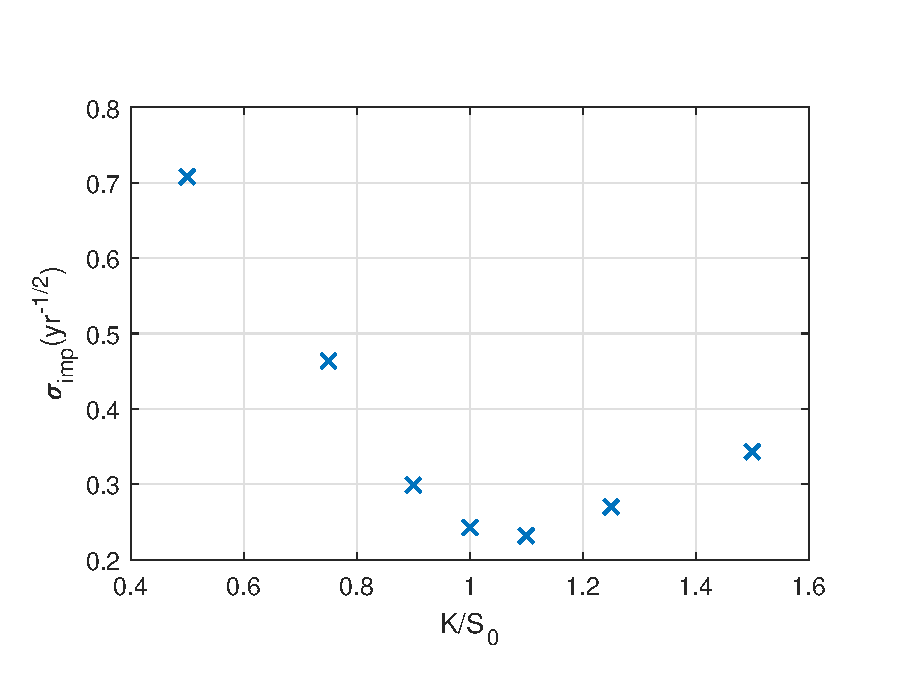
\includegraphics[width=0.49\linewidth,trim={0.25cm 0.45cm 1.1cm 1.4cm},clip]{T1.eps}}
    \subfigure[European Call Price, T=21 days]{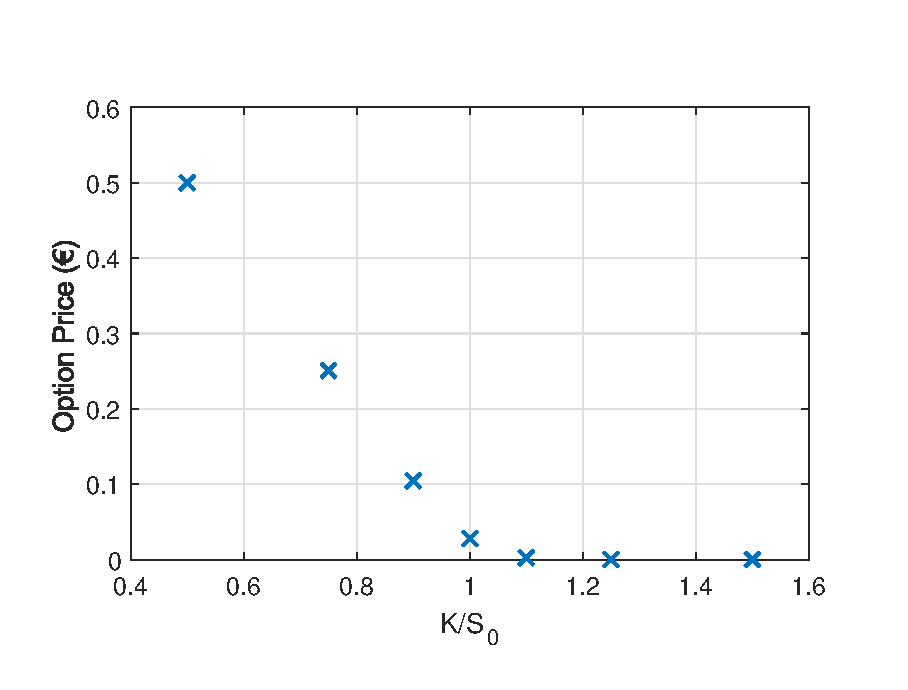
\includegraphics[width=0.49\linewidth,trim={0.25cm 0.45cm 1.1cm 1.4cm},clip]{T1P.eps}}
    \subfigure[Implied Volatility, T=42 days]{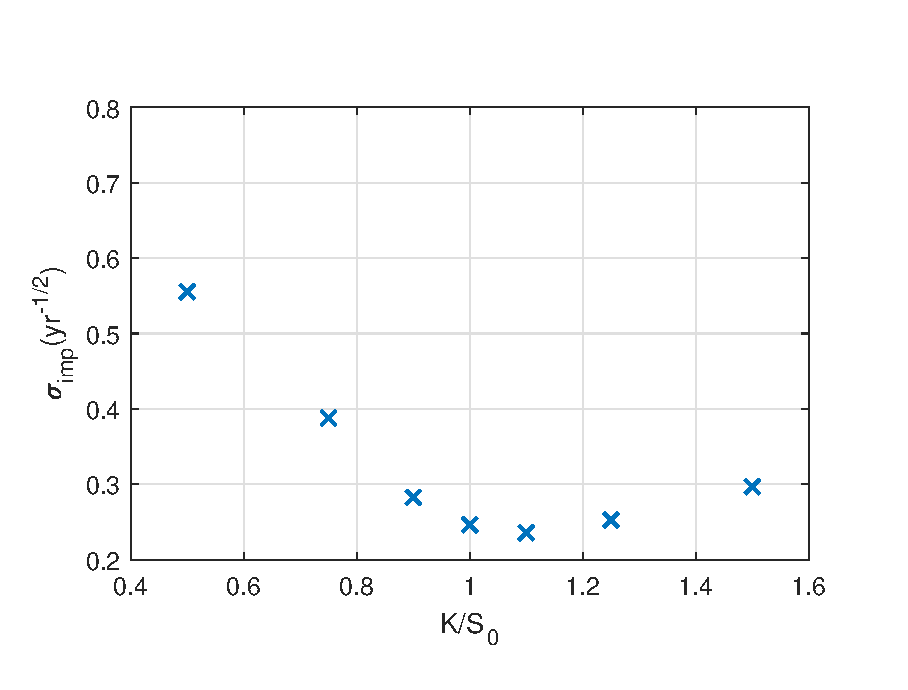
\includegraphics[width=0.49\linewidth,trim={0.25cm 0.45cm 1.1cm 1.4cm},clip]{T2.eps}}
    \subfigure[European Call Price, T=42 days]{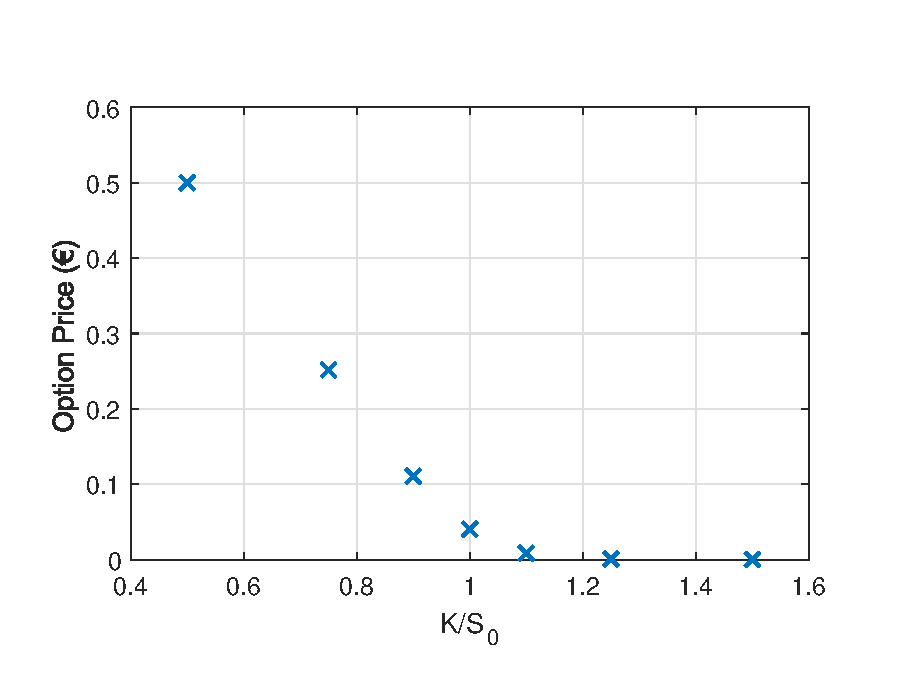
\includegraphics[width=0.49\linewidth,trim={0.25cm 0.45cm 1.1cm 1.4cm},clip]{T2P.eps}}
    \subfigure[Implied Volatility, T=63 days]{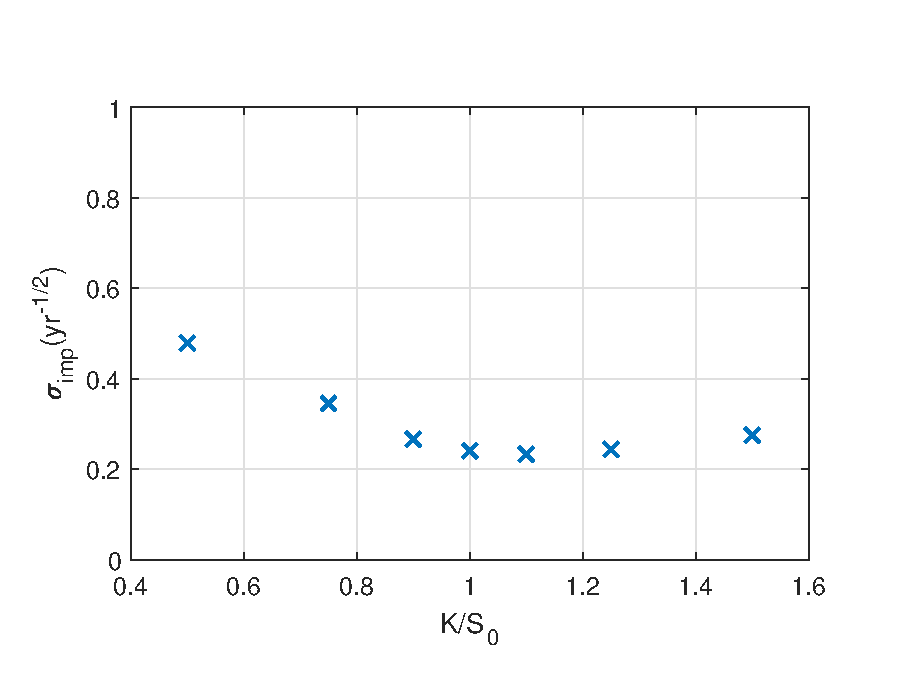
\includegraphics[width=0.49\linewidth,trim={0.25cm 0.45cm 1.1cm 1.4cm},clip]{T3.eps}}
    \subfigure[European Call Price, T=63 days]{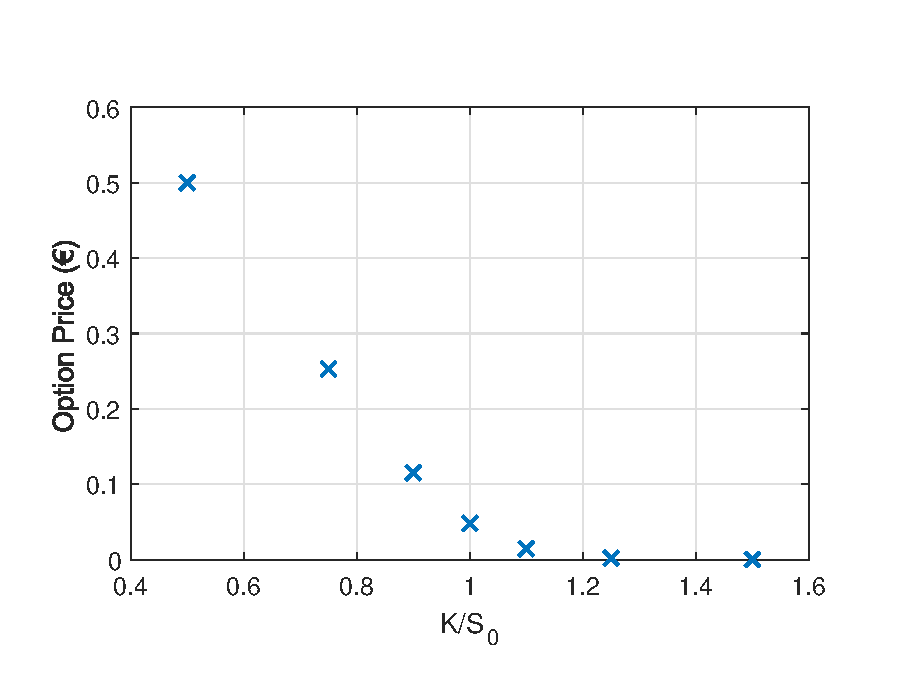
\includegraphics[width=0.49\linewidth,trim={0.25cm 0.45cm 1.1cm 1.4cm},clip]{T3P.eps}}
  \end{subfigmatrix}
  \caption[Scatter plots of the implied volatilities and European call prices provided, for 21, 42 and 63 days, to be used in model calibration and validation.]{Scatter plots of the implied volatilities and European call prices provided, for 21, 42 and 63 days, to be used in model calibration and validation.}
  \label{fig:mktdata}
\end{figure}

\begin{figure}[!htb]
  \begin{subfigmatrix}{2}
    \subfigure[Implied Volatility, T=126 days]{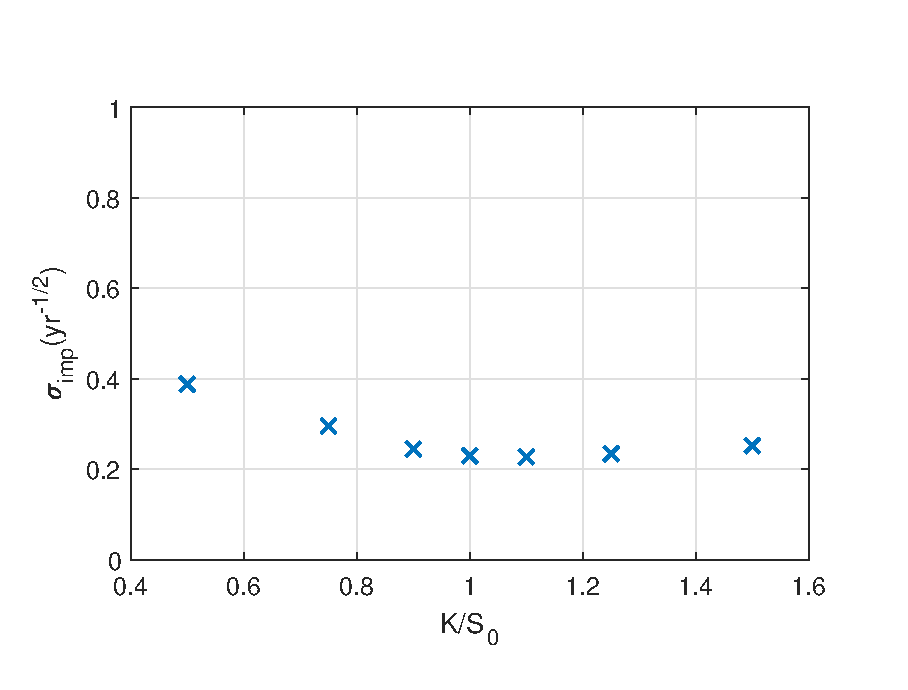
\includegraphics[width=0.49\linewidth,trim={0.25cm 0.45cm 1.1cm 1.4cm},clip]{T4.eps}}
    \subfigure[European Call Price, T=126 days]{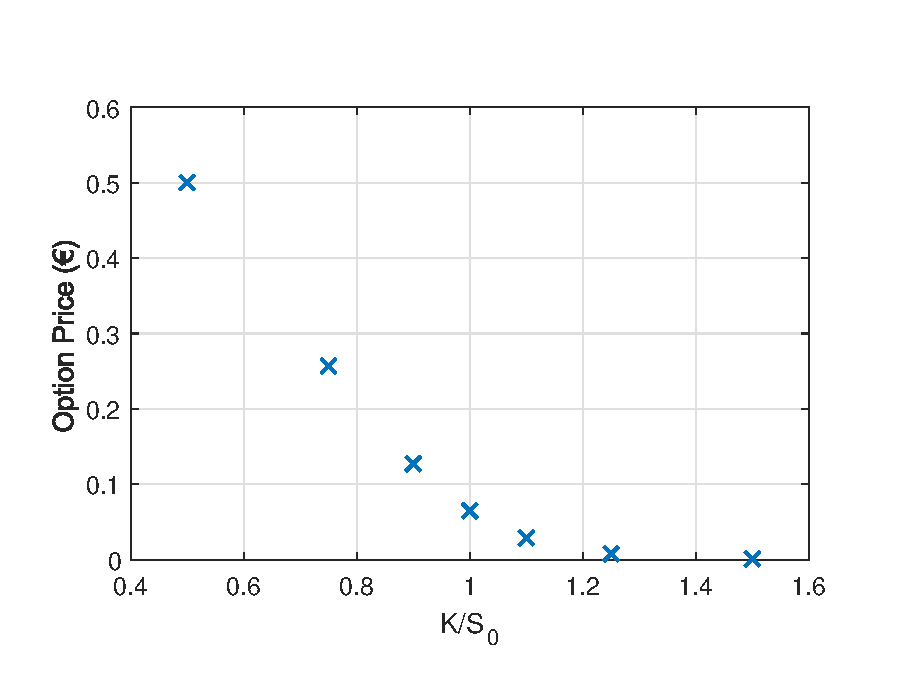
\includegraphics[width=0.49\linewidth,trim={0.25cm 0.45cm 1.1cm 1.4cm},clip]{T4P.eps}}
    \subfigure[Implied Volatility, T=189 days]{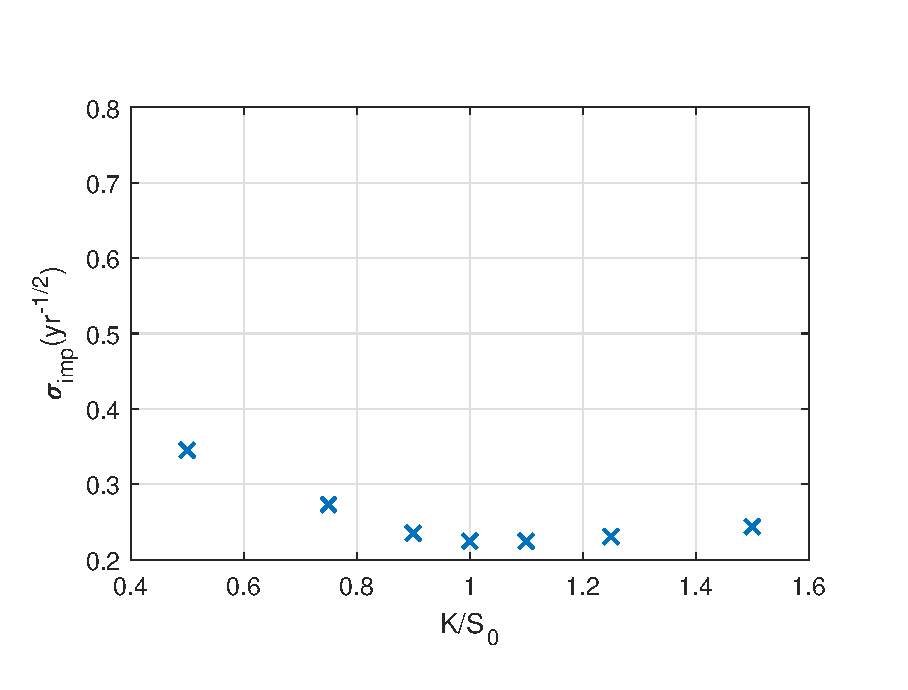
\includegraphics[width=0.49\linewidth,trim={0.25cm 0.45cm 1.1cm 1.4cm},clip]{T5.eps}}
    \subfigure[European Call Price, T=189 days]{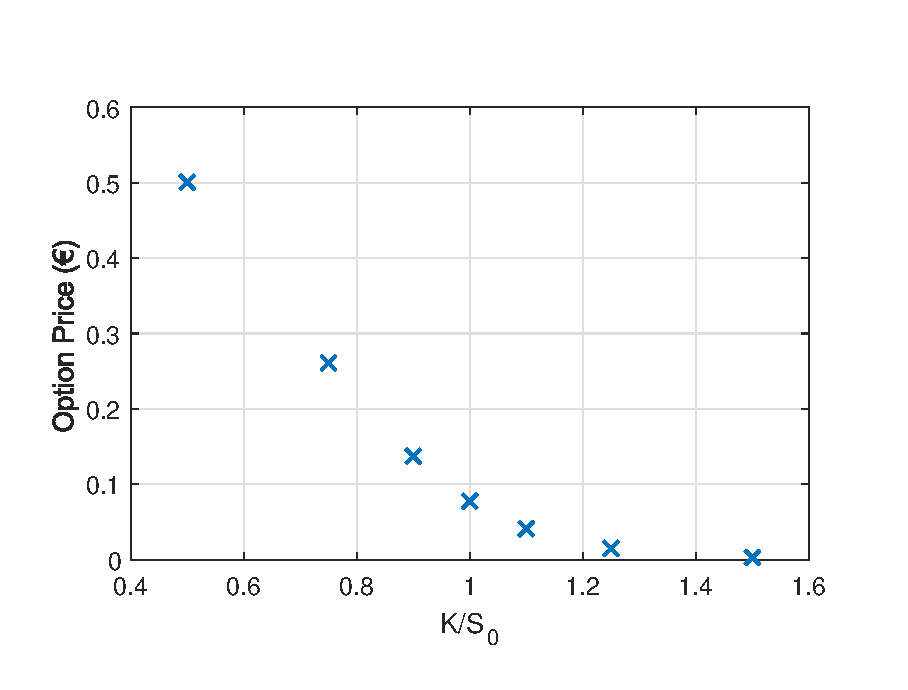
\includegraphics[width=0.49\linewidth,trim={0.25cm 0.45cm 1.1cm 1.4cm},clip]{T5P.eps}}
    \subfigure[Implied Volatility, T=252 days]{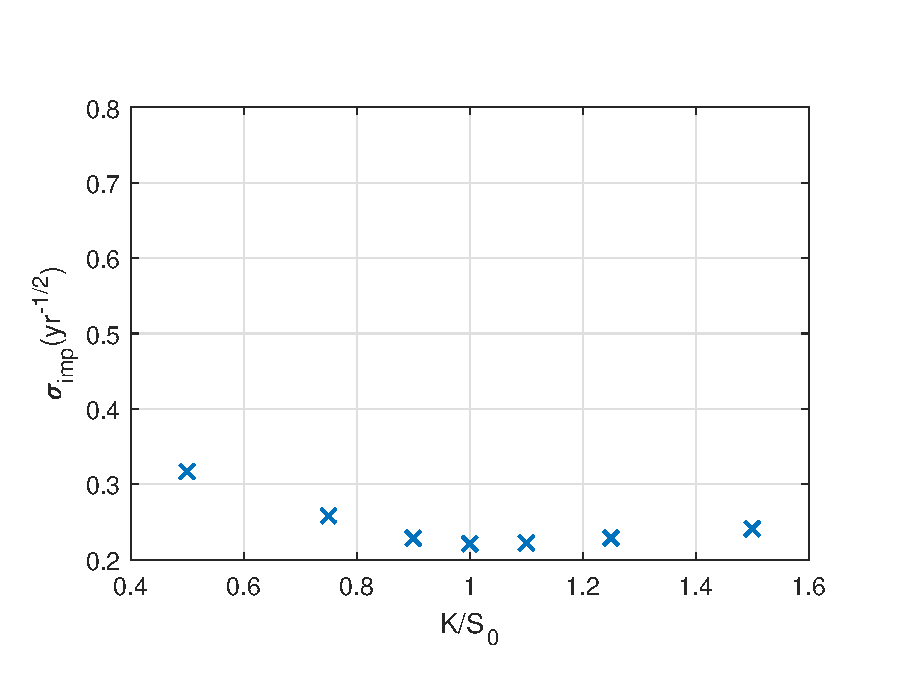
\includegraphics[width=0.49\linewidth,trim={0.25cm 0.45cm 1.1cm 1.4cm},clip]{T6.eps}}
    \subfigure[European Call Price, T=252 days]{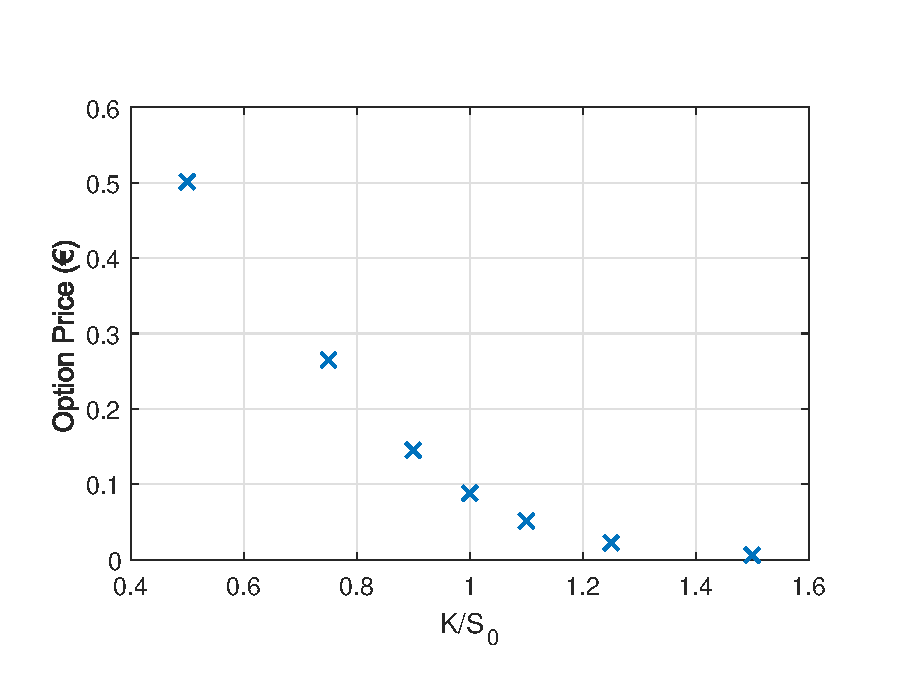
\includegraphics[width=0.49\linewidth,trim={0.25cm 0.45cm 1.1cm 1.4cm},clip]{T6P.eps}}
  \end{subfigmatrix}
  \caption[Scatter plots of the implied volatilities and European call prices provided, for 126, 189 and 252 days, to be used in model calibration and validation.]{Scatter plots of the implied volatilities and European call prices provided, for 126, 189 and 252 days, to be used in model calibration and validation.}
  \label{fig:mktdata2}
\end{figure}

